% Chapter Template

\chapter{Ensayos y resultados} % Main chapter title

En este capítulo se menciona los ensayos realizados asi como 

\label{Chapter4} % Change X to a consecutive number; for referencing this chapter elsewhere, use \ref{ChapterX}

%----------------------------------------------------------------------------------------
%	SECTION 1
%----------------------------------------------------------------------------------------

\section{Generación del sistema de pruebas}
\label{sec:pruebasHW}

La idea de esta sección es explicar cómo se hicieron los ensayos, qué resultados se obtuvieron y analizarlos.
\section{Pruebas unitarias}
\subsection{Pruebas del servidor Mosquitto}
Para simular mensajes y observar el comportamiento de cada una de las partes del sistema se utilizó la herramienta MQTT explorer   \citep{WEBSITE:29}.

\begin{figure}[ht]
	\centering
	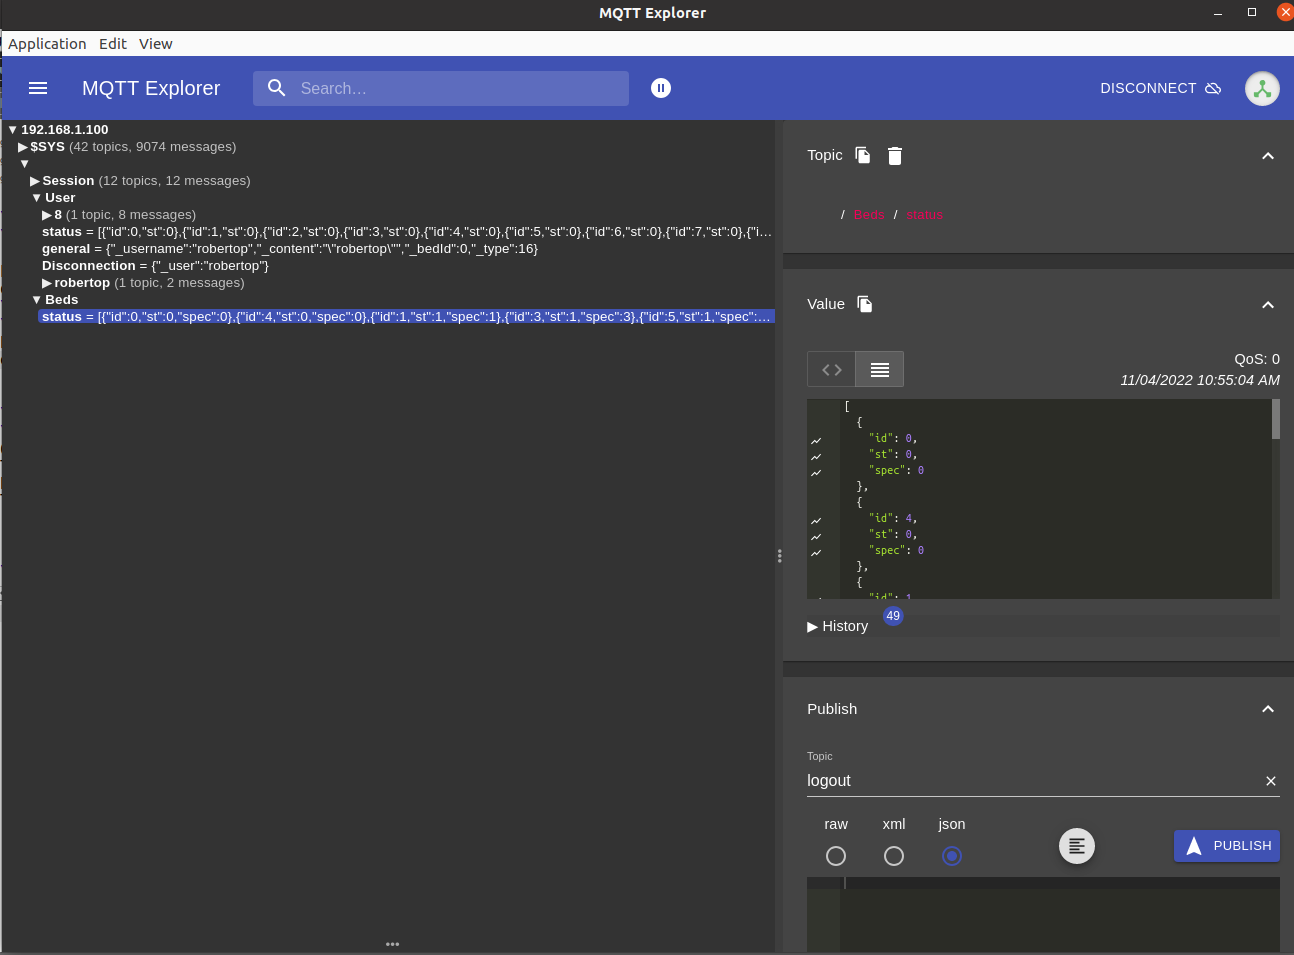
\includegraphics[scale=.25]{./Figures/mqtt-explorer.png}
	\caption{Imagen de MQTT Explorer.}
	\label{fig:MQTT Explorer}
\end{figure}

Esta herramienta fue no solo muy útil para realizar ensayos sino tambien para realizar el desarrollo de las funcionalidades propiamente dichas.

\subsection{Pruebas unitarias de la API Rest}

Para simular el logeo y la consulta a la base de datos se utilizó la herramienta PostMan \citep{WEBSITE:30} y la consola de administrador de phpMyAdmin mencionada en \ref{Chapter2}. En la \ref{fig:Logueo en el sistema con Postman} se observa el \textit{token} devuelto por el backend al logearse con las credenciales correspondientes y en \ref{fig:Rechazo Logueo en el sistema con Postman} se observa la respuesta al ingresar una contraseña inadecuada.

\begin{figure}[ht]
	\centering
	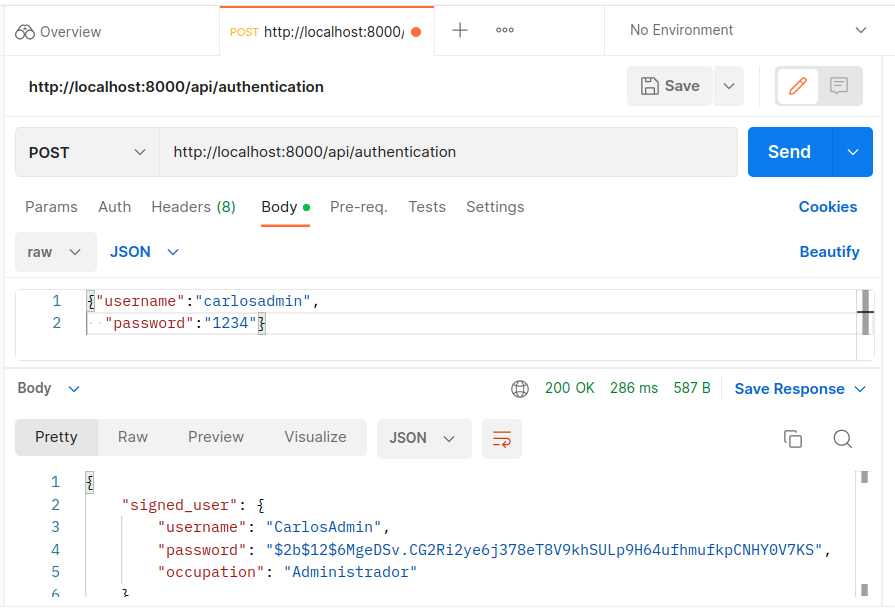
\includegraphics[scale=.35]{./Figures/auth.png}
	\caption{Logueo en el sistema con Postman.}
	\label{fig:Logueo en el sistema con Postman}
\end{figure}

\begin{figure}[ht]
	\centering
	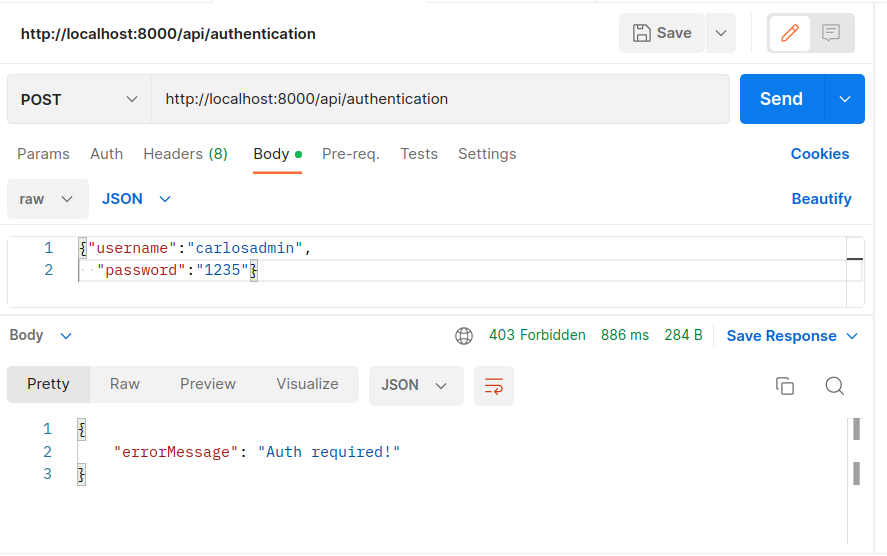
\includegraphics[scale=.35]{./Figures/no-auth.png}
	\caption{Rechazo de logueo.}
	\label{fig:Rechazo Logueo en el sistema con Postman}
\end{figure}


Durante el desarrollo, se deshabilitó la opción de logueo para facilitar las pruebas. 

\section{Integración del sistema}
\subsection{Instalación del sistema en una instancia de AWS}
Con el objetivo de no incorporar costos en las pruebas, se generó una instancia Free Tier en Amazon Web Services, en la cual se instaló Ubuntu, el broker Mosquitto, el backend, la página Web y un servidor NGINX para que funcione como proxy inverso. Tambien se contrató el servicio route 53 que permite customizar las politicas de ruteo.
De esta manera, se puede acceder al sistema desde cualquier dispositivo móvil conectado a una red.
Los pasos para configurar el sistema backend en la instancia EC2 con ubuntu consisten en:

\begin{itemize}
\item Logearse en la instancia con ssh.
\item Instalar el Git:

	''sudo apt-get install git''
\item Instalar el broker Mosquitto:
	
	''sudo apt-get install mosquitto''
\item Configurar según \ref{Broker Mosquitto}.
\item Instalar Docker y Docker-compose
\item Descargar el backend desde GitHub
\item Copiar en la instancia la base de datos comprimida y descomprimir dentro de la carpeta /db
\item Ejecutar Docker-compose up
\end{itemize}

Los pasos para configurar la página web:
\begin{itemize}
\item Compilar la página web: dentro de el proyecto ejecutar:

''ionic build''
\item Comprimir la carpeta www
\item Logearse con ssh en la instancia EC2

\end{itemize}
\subsection{Generación/instalación de la aplicación móvil en ANDROID}

Para poder descargar el archivo ejecutable a un dispositivo ANDROID se debe generar el archivo .apk correspondiente. Para ello seguir los siguientes pasos:

\begin{itemize}
\item Generar código con ionic capacitor:

''ionic cap build android''
\item Abrir Android estudio, modificar el AndroidManifest.xml
\item Generar el bundle o en su defecto, conectar el celular en modo debug y descargar la aplicación.
\end{itemize}
\pagebreak


\begin{lstlisting}[label=cod:AndroidMan,caption=Modificaciones al Android Manifest.]  % Start your code-block
package="com.gabiot.Enfermera">
    <!-- Permissions -->

    <uses-permission android:name="android.permission.INTERNET" />
    <uses-permission android:name="android.permission.READ_EXTERNAL_STORAGE" />
    <uses-permission android:name="android.permission.WRITE_EXTERNAL_STORAGE" />
    <uses-permission android:name="android.permission.ACCESS_NETWORK_STATE" />
    <uses-permission android:name="android.permission.ACCESS_WIFI_STATE" />

    <uses-permission android:name="android.permission.WAKE_LOCK" />
    <uses-permission android:name="android.permission.READ_PHONE_STATE" />
    <uses-permission android:name="android.permission.CAMERA" />
    <uses-sdk tools:overrideLibrary="com.google.zxing.client.android" />
    <uses-permission android:name="android.permission.RECORD_AUDIO" />

    <application
        android:allowBackup="true"
        android:icon="@mipmap/ic_launcher"
        android:label="Enfermera"
        android:roundIcon="@mipmap/ic_launcher_round"
        android:supportsRtl="true"
        android:theme="@style/AppTheme"
        android:usesCleartextTraffic="true"
        android:hardwareAccelerated="true">
        <!-- Mqtt Service -->
        <service
            android:enabled="true"
            android:name="org.eclipse.paho.android.service.MqttService"
            android:exported="false"
        />
...

\end{lstlisting}
\pagebreak
\subsection{Equipo simulador de llamadores}

Se desarrollo un dispositivo que simula los llamadores con un microcontrolador ESP32, una fuente y un teclado matricial. Presionando una tecla, genera un evento en MQTT. El código y el esquemático del mismo se encuentra en \citep{WEBSITE:33} 

\begin{figure}[ht]
	\centering
	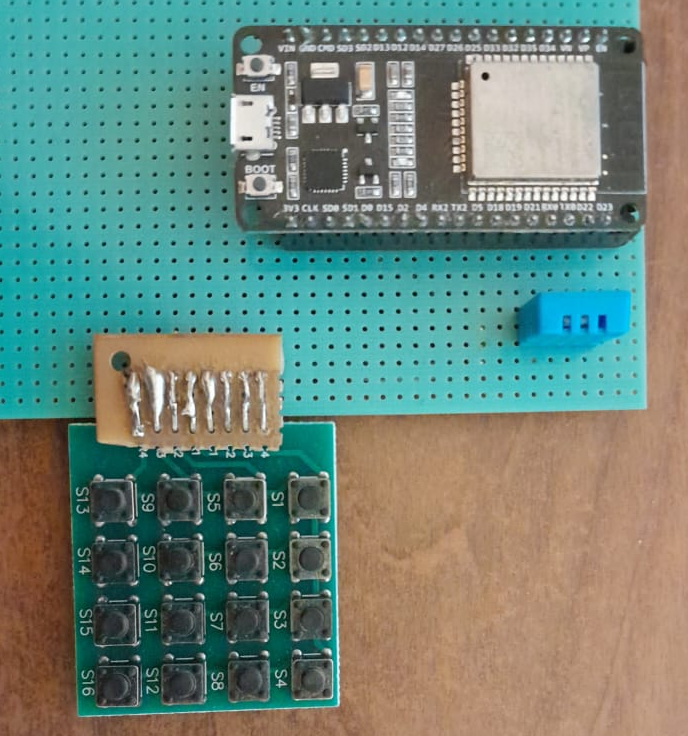
\includegraphics[scale=.35]{./Figures/simulador.png}
	\caption{Simulador de llamadores.}
	\label{fig:Simulador de llamadores}
\end{figure}

\subsection{Resultados de utilizar el sistema}

El sistema permaneció funcionando de manera normal durante una semana completa, generando los eventos programados y permitiendo la interacción de dispositivos.
